\subsection{El reparto}
\subsubsection{Protocolo de reparto de cartas}
El siguiente es el protocolo que da como resultado tres cartas para cada jugador elegidas de forma azaroza.

\begin{figure}
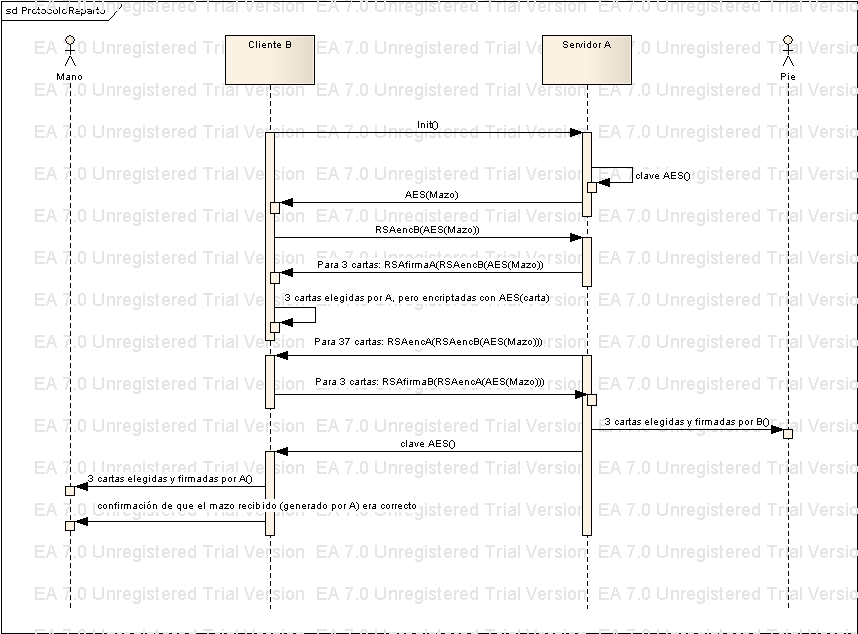
\includegraphics{ProtocoloReparto.png}
\end{figure}

Notar que cuando se hace referencia a RSA no es estrictamente al algoritmo RSA, sino a la variante que utiliza un m'odulo primo descripta en Mental Poker, y que en ning'un momento hay intercambio de claves de algoritmos asim'etricos. La 'unica clave transmitida es la utilizada por AES.
En este caso "firmar" equivale a encriptar y enviar a la otra parte tanto el plaintext como el encriptado. En este esquema, el firmate es el 'unico que puede validar su firma, pero esto es suficiente si lo que se desea es validar que la carta jugada por el oponente sea una de las que uno mismo le reparti'o.

\begin{enumerate}

\item B le pide conexi'on a A

\begin{verbatim}

------------
|  "INIT"  |
------------
4 bytes

\end{verbatim}




\item A genera una clave sim'etrica $k$ (por ejemplo, con AES), encripta las 40 cartas $M_1...M_40$ con $k$ y las env'ia a B ($k$ sirve para asegurar que el mazo enviado por A en este paso es v'alido).

\begin{verbatim}

------------------------------------------------
|   k(M1)   |   k(M2)   |   ...   |   k(M40)   |
------------------------------------------------
  160 bits    160 bits               160 bits

\end{verbatim}

  


\item B genera un $p$ primo grande y genera $e^1_b$, $d^1_b$ (utilizadas para asegurar un reparto justo) y  $e^2_b$, $d^2_b$ (utilizadas para asegurar que se jueguen las cartas repartidas) tal que

$$	e^1_b * d^1_b = 1 [mod\ p-1] = e^2_b * d^2_b $$

Env'ia a A el $p$ y las cartas ya encriptadas con $k$ encriptadas a su vez con $e^1_b$ (usando RSA)

$$	e^1_b(k(M_i)) = k(M_i)^{e^1_b} $$
	

\begin{verbatim}
-----------------------------------------------------------------------
|   p   |   e1b(k(M1))   |   e1b(k(M2))   |   ...   |   e1b(k(M40))   |
-----------------------------------------------------------------------
  1024 b     1024 b           1024 b         1024 b       1024 b       
\end{verbatim}


  


\item A usa $p$ para generarse sus propias claves

$$	e^1_a * d^1_a = 1 [mod\ p-1] = e^2_a * d^2_a $$

Elige al azar 3 cartas de las enviadas por B ($B_1, B_2, B_3$) y las firma con $e^2_a$. Env'ia cada carta como una tupla

$$	<e^1_b(k(Bi)), 			e^2_a(e^1_b(k(Bi)))> = 
	<k(Bi)^{e^1_b} [mod\ p], 	k(Bi)^(e^1_b * e^2_a) [mod\ p]> $$
	
A su vez, repite el paso anterior realizado por B envi'andole a este el resto de las cartas (Ri) encriptadas con su clave:

$$	e^1_a(e^1_b(k(Ri))) = k(Ri)^(e^1_b * e^1_a) [mod\ p] $$
	

\begin{verbatim}
--------------------------------------------------------------------------
|   e1b(k(B1))   |   e1b(k(B2))   |   e1b(k(B3))   |   e2a(e1b(k(B1)))   |
--------------------------------------------------------------------------
     1024 b           1024 b           1024 b              1024 b         

--------------------------------------------
   e2a(e1b(k(B2)))   |   e2a(e1b(k(B3)))   |
--------------------------------------------
       1024 b                1024 b         

------------------------------------------------------------------------------
|    e1a(e1b(k(R1)))   |   e1a(e1b(k(R2)))   |   ...   |   e1a(e1b(k(R37)))  |
------------------------------------------------------------------------------
        1024 b                1024 b                         1024 b           
\end{verbatim}
	
	
	
	
	
\item B recibe sus cartas (las tuplas) y les aplica la desencripci'on de $e^1_b$ con $d^1_b$:

$$	<d^1_b(k(B_i)^{e^1_b} [mod\ p]), 		d^1_b(k(B_i)^{e^1_b * e^2_a} [mod\ p])> = $$
$$	<k(B_i)^{e^1_b * d^1_b} [mod\ p], 	k(B_i)^{e^1_b * e^2_a * d^1_b} [mod\ p]> = $$
$$	<k(B_i), 						k(B_i)^{e^2_a} [mod\ p]> $$

A su vez, elige 3 cartas al azar ($A_1, A_2, A_3$) del resto (las $R_i$) y les aplica tambi'en $d^1_b$:
	
$$	d^1_b(k(A_i)^{e^1_b * e^1_a} [mod\ p]) = 
	k(A_i)^{e^1_b * e^1_a * d^1_b} [mod\ p] =
	k(A_i)^{e^1_a} [mod\ p] $$

Para completar la mano de A, debe completar las tuplas con su firma:

$$	e^2_b(k(A_i)^{e^1_a} [mod\ p]) =
	k(A_i)^{e^1_a * e^2_b} [mod\ p] $$
	
y se las env'ia a A:

$$	<k(A_i)^{e^1_a} [mod\ p],			k(A_i)^{e^1_a * e^2_b} [mod\ p]> $$
	

\begin{verbatim}
--------------------------------------------------------------------------
|   e1a(k(A1))   |   e1a(k(A2))   |   e1a(k(A3))   |   e2b(e1a(k(A1)))   |
--------------------------------------------------------------------------
     1024 b           1024 b           1024 b              1024 b         

--------------------------------------------
   e2b(e1a(k(A2)))   |   e2b(e1a(k(A3)))   |
--------------------------------------------
       1024 b                1024 b         
\end{verbatim}
	
	
	
	
	
\item A recibe sus cartas y les aplica la desencripci'on de $e^1_a$ con $d^1_a$:

$$	<d^1_a(k(A_i)^{e^1_a} [mod\ p]),			d^1_a(k(A_i)^{e^1_a * e^2_b} [mod\ p])> = $$
$$	<k(A_i)^{e^1_a * d^1_a} [mod\ p],			k(A_i)^{e^1_a * e^2_b * d^1_a} [mod\ p]> = $$
$$	<k(A_i),								k(A_i)^{e^2_b} [mod\ p]> $$
	
A utiliza $k$ para ver las cartas que le tocaron, su mano queda

$$	<A_i, k(A_i)^{e^2_b} [mod\ p]> $$

Por 'ultimo, envia $k$ a B


\begin{verbatim}
---------
|   k   |
---------
  128 b
\end{verbatim}

	 
	 
	 


\item B recibe $k$, con lo que la utiliza para ver los $M_i$ que le mando A en el paso 2 (poseia $k(M_i)$) y verificar que le mand'o un mazo valido. Tambi'en desencripta su mano para ver las cartas que le tocaron:

$$	<B_i, k(B_i)^{e^2_a} [mod\ p]> $$
	
\end{enumerate}	




\subsubsection{Pre-inicio del juego}
Este es final del inicio del juego. Se setean datos para ser usados durante el resto de la mano.

\begin{enumerate}
\item Ahora que ambos tienen sus manos, B se genera un par de claves RSA comunes y corrientes 

$$	(e^3_b, n_b), (d^3_b, n_b)  $$
	
y env'ia la p'ublica $(e^3_b, n_b)$ a A. Usar'a $d^3_b$ s'olo para firmar sus acciones.

A su vez, genera un paquete con el timestamp inicial decretando esta como la hora de inicio de juego. Lo env'ia firmado con $d^3_b$.

\begin{verbatim}
------------------------------------
|   e3b   |   nb   |   d3b(ts_i)   |
------------------------------------
  2048 b    2048 b      2048 b
\end{verbatim}
  
  
  


\item A lee con la clave p'ublica de B lo firmado por 'el y verifica que el timestamp es v'alido. Se genera tambi'en sus pares de claves RSA

$$	(e^3_a, n_a), (d^3_a, n_a) $$
	
y env'ia su aceptaci'on (firmada con $d^3_a$) de la hora de inicio.


\begin{verbatim}
--------------------
|   e3a   |   na   |
--------------------
  2048 b    2048 b  
\end{verbatim}
  
  


\item Al recibir B la verificaci'on, puede empezar a jugar (notar que es mano).

\end{enumerate}
